\documentclass[conference]{IEEEtran}
\usepackage[T1]{fontenc}
\usepackage{amsmath,amssymb}
\usepackage{graphicx}
\usepackage{xcolor}
\usepackage{tikz}
\usetikzlibrary{shapes.geometric,arrows.meta,positioning,fit}
\usepackage{booktabs}
\usepackage{multirow}
\usepackage{url}

\newcommand{\TBD}{\textcolor{red}{\textbf{[TBD]}}}
\newcommand{\code}[1]{\texttt{#1}}

\begin{document}

\title{Vehicle Classification, Multi-Object Tracking and Counting, and
Speed Estimation on a Grid-Based Motion-Detection Baseline: Sequential
and Parallel Implementations with a Fair-Comparison Evaluation}

\author{
\IEEEauthorblockN{Jay Suriya R}
\IEEEauthorblockA{Department of Computer Science and Engineering\\
Indian Institute of Information Technology Sri City\\
Sri City, India\\
jaysuriya.r24@iiits.in}
\and
\IEEEauthorblockN{Manipriya Sankaranarayanan}
\IEEEauthorblockA{Department of Computer Science and Engineering\\
Indian Institute of Information Technology Sri City\\
Sri City, India\\
manipriya.s@iiits.in}
}

\maketitle

\begin{abstract}
A prior published system \cite{baseline} performs grid-based vehicle
motion detection: a region of interest (ROI) is discretized into a
grid, histogram-equalized frame differencing marks each cell as
motion/no-motion, and a preliminary dual-ROI implementation dispatches
this per-cell work across a thread pool created anew every frame. Its
released implementation stops at a binary occupancy grid: it does not
classify vehicles, track individual vehicles across frames, count line
crossings, estimate speed, or evaluate against ground truth. This paper
builds that layer on top of the baseline's motion-detection front end
-- rule-based vehicle classification from per-cluster grid geometry,
multi-object tracking with temporally smoothed labels and
duplicate-aware line-crossing counting, displacement-gated speed
estimation, and adaptively thresholded traffic-density estimation --
in a sequential form and in a redesigned parallel form that keeps all
per-lane state in a \code{LaneTracker} class, uses two persistent
\code{ThreadPoolExecutor} pools, and separates state updates from drawing
on the shared frame. A cross-implementation check -- comparing per-video
UA-DETRAC confusion matrices of the sequential implementation and the
parallel implementation's first lane -- surfaced two real preprocessing
divergences (a missing pre-differencing Gaussian blur, and a
histogram-equalization step that discarded color information). After
fixing both, the two implementations produce matching confusion matrices
and F1 scores on all 12 tested videos (drawn from UA-DETRAC's
Cloudy/Night/Rainy/Sunny categories across three density tiers). We then
time four workloads on a 4-core/8-thread laptop CPU: sequential one-lane,
threaded one-lane, the same two-lane code without threads, and threaded
two-lane. Threading does \emph{not} reduce execution time on this
machine: for the same two-lane workload the threaded run is slower than
the unthreaded one (time ratio $0.860\pm0.077$, slower on all 12 videos;
mean $\pm$ between-video std). The workload-normalized ROI-frame
throughput of the threaded two-lane run relative to the sequential
one-lane run is $1.257\pm0.228$, but processing two lanes without any
threads already gives $1.458\pm0.216$: the gain comes from sharing
once-per-frame work between lanes, not from threading. Even the
single-threaded Python script keeps about four cores busy through native
multithreading inside OpenCV, which leaves Python-level threads little to
add; Amdahl ceilings at the lane-pool width of 2 (1.22 when $p$ counts
the work dispatched to the pool, 1.50 for the seven largest native calls)
are not approached. Normalized throughput correlates weakly and
negatively with traffic density ($r{=}-0.45$), while the tracking stage
takes only 1.6--4.2\% of run time with no density trend. We report full
accuracy and timing breakdowns and document the benchmarking artifacts
and algorithmic divergences found along the way as evidence for a
general point: ``identical algorithm, parallelized'' and ``parallel is
faster'' are empirical claims that must be measured, not assumed.
\end{abstract}

\begin{IEEEkeywords}
vehicle classification, multi-object tracking, vehicle counting, speed
estimation, traffic density estimation, parallel computing, thread
pool, Python GIL, UA-DETRAC
\end{IEEEkeywords}

\section{Introduction}
\label{sec:intro}

Automated traffic monitoring increasingly relies on video analytics:
existing road cameras can support vision-based vehicle counting and
classification without dedicated inductive-loop or radar hardware
\cite{crouzil2016}. Recent vehicle-monitoring systems combine learned
detectors with multi-object trackers, e.g.\ YOLOv7 with DeepSORT
\cite{lian2025} or an improved YOLOv8 with BoT-SORT \cite{liu2025}.
Model complexity, parameter count, power and throughput are recognized
deployment challenges for such systems on edge hardware \cite{zhai2023};
lightweight architectures and quantization reduce these demands
\cite{chang2025,macko2025}. Classical foreground-segmentation pipelines
remain a practical, training-free alternative for counting and coarse
classification \cite{unzueta2012}, although illumination changes,
shadows, camera placement and occlusion make them fragile
\cite{abbas2021,chen2020}.

\subsection{Relationship to Prior Published Work}
\label{sec:priorwork}
A previously published system, Two-Tier Parallel Virtual Lattice Layers
(TPL2) \cite{baseline}, addresses the motion-detection front end of this
problem without a learned detector: each region of interest (ROI) is
discretized into a grid; consecutive frames are histogram-equalized and
differenced; and each grid cell is independently marked motion/no-motion
via per-cell blur-threshold-dilate-contour detection, with per-cell and
per-lane work dispatched to a \code{ThreadPoolExecutor}. The TPL2 paper
also describes a lattice-run heuristic for counting vehicles (its
Eqs.~7--8) and density derived from those counts, leaves tracking-based
speed estimation to future work, and reports execution time and memory
-- an efficiency improvement of about 26.55\% with a 3.72\% memory
increase -- but no detection-accuracy metrics
\cite{baseline,muthuraja2026}. Its released implementation, on which this
work builds, stops at a binary per-cell occupancy grid (printing the raw
occupancy fraction): it contains no vehicle-type classification, no
per-vehicle tracking or identity assignment, no line-crossing counting,
no speed estimation, no adaptively thresholded density estimation and no
evaluation against ground truth, and its parallel variant creates a new
thread pool every frame and stores no persistent per-lane tracking
state. Section~\ref{sec:overview} describes this baseline in the detail
needed to fix notation, and Table~\ref{tab:baseline-vs-contribution}
summarizes the boundary.

This paper documents what is built on top of that occupancy grid:
rule-based vehicle classification from the geometry of clustered hot
cells; multi-object tracking with temporally smoothed labels,
duplicate-track suppression, and duplicate-crossing-aware vehicle
counting; displacement-gated speed estimation; and adaptively
thresholded traffic-density estimation combining spatial occupancy with
recent flow -- implemented and evaluated in \emph{both} a sequential
form and a parallel form. Per-vehicle tracking, label smoothing and
speed estimation need state that persists across frames for each lane;
the parallel form therefore introduces per-lane \code{LaneTracker}
instances that hold this state and persistent thread pools
(Section~\ref{sec:parallel}), rather than reusing the baseline's
per-frame threading.

We implement and document two versions of the resulting system:

\begin{itemize}
\item \textbf{Sequential (\code{seq.py})}: a single-lane, procedural
implementation using module-level global state, instrumented with
per-frame timing, memory sampling, and \code{cProfile}-based
function-level profiling.
\item \textbf{Parallel (\code{rparallel\_he3.py})}: a dual-lane
implementation that encapsulates all per-lane tracking state in a
\code{LaneTracker} class and dispatches (i) the $O(\text{rows}\times
\text{cols})$ per-cell contour computations and (ii) the two lanes'
grid-detection and tracking-state updates across two persistent
\code{ThreadPoolExecutor} pools.
\end{itemize}

The two implementations are intended to be algorithmically identical in
every stage except lane count -- but, as Section~\ref{sec:crosscheck}
reports, that intended equivalence was not automatic and had to be
verified and repaired. Comparing them also introduces a workload
confound (one ROI vs.\ two ROIs per frame) that a naive wall-clock
comparison would silently absorb into an inflated or deflated
``speedup'' number. Section~\ref{sec:experiments} makes this confound
explicit, defines a workload-normalized throughput metric, and adds
same-workload baselines that isolate the effect of threading itself.

\begin{table}[t]
\centering
\caption{What is prior published work \cite{baseline} vs.\ this
paper's contribution.}
\label{tab:baseline-vs-contribution}
\footnotesize
\begin{tabular}{p{3.9cm}p{3.6cm}}
\toprule
\textbf{Prior work \cite{baseline} (baseline)} & \textbf{This paper} \\
\midrule
ROI grid discretization &
Spatial clustering of hot cells into vehicle-sized objects
(Section~\ref{sec:cluster}) \\
Per-cell motion detection (blur/threshold/dilate/contour) &
Retuned per-cell detection parameters to support geometric classification
(Section~\ref{sec:motion}) \\
Histogram-equalized frame differencing &
-- (reused; two latent bugs in it found and fixed, Section~\ref{sec:crosscheck}) \\
-- &
Rule-based vehicle classification (Section~\ref{sec:classify}) \\
Lattice-run vehicle-count heuristic (paper only) &
Multi-object tracking, duplicate suppression, line-crossing counting
(Section~\ref{sec:tracking}) \\
Speed estimation left to future work &
Displacement-gated speed estimation (Section~\ref{sec:speed}) \\
Raw occupancy fraction (code); count-based density (paper) &
Adaptive percentile-based density thresholding with flow blending
(Section~\ref{sec:density}) \\
Thread pool created every frame; no persistent per-lane state &
Persistent two-pool architecture with per-lane
\code{LaneTracker} state (Section~\ref{sec:parallel}) \\
Execution time and memory only &
DETRAC ground-truth evaluation methodology (Section~\ref{sec:eval}) \\
-- &
Four-workload benchmarking protocol and cross-implementation
validation (Sections~\ref{sec:experiments}--\ref{sec:crosscheck}) \\
\bottomrule
\end{tabular}
\end{table}

This work builds on that baseline through five contributions:
1) a rule-based vehicle classification, multi-object tracking and
counting, and speed-estimation layer, together with every hand-tuned
constant that governs its behavior (Table~\ref{tab:params}),
implemented identically in both a sequential and a parallel execution
model; 2) an adaptively thresholded traffic-density estimator that
extends the baseline's raw per-frame occupancy fraction with
percentile-based recalibration and flow blending
(Section~\ref{sec:density}); 3) a redesigned concurrency architecture --
two persistent thread pools and per-lane \code{LaneTracker} state --
introduced because the new layer needs cross-frame state per lane that
the baseline does not store (Section~\ref{sec:parallel}), together with
measurements showing that on the evaluated machine this threading does
not reduce execution time; 4) a DETRAC-grounded evaluation methodology
covering both grid-level and vehicle-level (ID-based) accuracy, applied
identically to both implementations (Section~\ref{sec:eval}); and 5) a
benchmarking protocol and orchestration script
(\code{benchmarking/orchestrate\_benchmark.py}) that times four
workloads -- separating the effect of the workload (one vs.\ two lanes)
from the effect of threading -- together with a cross-implementation
validation methodology that found and fixed two accuracy-affecting
divergences in the reused preprocessing step before any comparison was
trusted (Sections~\ref{sec:experiments}--\ref{sec:crosscheck}).

\section{Related Work}
\label{sec:related}

The grid-based motion-detection front end this paper builds on --
ROI discretization, histogram-equalized frame differencing, and
per-cell blur-threshold-dilate-contour occupancy detection, together
with a preliminary dual-ROI threaded implementation -- is prior
published work \cite{baseline}. This paper does not re-claim that
front end; Section~\ref{sec:overview} and Table~\ref{tab:baseline-vs-contribution}
describe it only to the extent needed to establish notation, and every
subsequent section is explicit about which parts are reused unchanged,
which are retuned, and which are new.

Frame differencing and background subtraction remain widely used for
motion detection in traffic video because of their low computational
cost relative to learned detectors. Cheung and Kamath compare simple
frame-differencing and adaptive median filtering against more elaborate
probabilistic background models for urban traffic video and find that
the simpler techniques remain competitive at a fraction of the
computational cost \cite{cheung2004}; Unzueta et al.\ demonstrate
real-time vehicle counting and classification with adaptive multicue
background subtraction \cite{unzueta2012}, and Crouzil et al.\ a
counting system built on existing traffic cameras \cite{crouzil2016}.
Such pipelines are sensitive to camera position, background variation
and occlusion \cite{abbas2021} and to sudden illumination changes and
shadows \cite{chen2020}, which motivates the contrast normalization used
here (Section~\ref{sec:motion}) and bounds what can be expected of it
(Section~\ref{sec:threats}). Contour extraction from the resulting binary
motion masks -- used throughout the baseline and this paper via OpenCV's
\code{cv2.findContours} -- follows the border-following algorithm of
Suzuki and Abe \cite{suzuki1985}.

A separate, contemporaneous extension of the same baseline
\cite{muthuraja2026} pursues a complementary direction: scene-adaptive
preprocessing (per-frame illumination classification, CLAHE, and a Dark
Channel Prior degradation indicator) and perspective-aware centroid
non-maximum suppression, evaluated on 60 UA-DETRAC sequences with a
Hungarian-matched protocol and reporting 71.03\% micro-averaged F1. That
work notes that the baseline ``reports execution time and memory
consumption but does not provide detection-accuracy metrics,'' and adds
an accuracy evaluation without addressing parallelization. The present
paper is complementary in the other direction: it adds no scene-adaptive
preprocessing, but adds vehicle classification, multi-object tracking
and counting, speed estimation, and a verified-equivalent
sequential/parallel comparison methodology.

For tracking, SORT combines Kalman-filter motion prediction with
Hungarian assignment for efficient online tracking \cite{bewley2016}, and
DeepSORT adds appearance association to improve robustness under
occlusion \cite{wojke2017}; this paper uses simpler greedy
nearest-centroid association (Section~\ref{sec:tracking}) and lists
these methods as future alternatives. Pixel-displacement speed estimates
require an appropriate image-to-metric scale, e.g.\ via homography
rectification, and validation against measured speeds \cite{kamil2024},
and unstable detected trajectories are a recognized source of speed error
\cite{sangsuwan2024}.

Evaluation is performed against the UA-DETRAC benchmark, a large-scale
traffic video dataset with per-frame, per-vehicle bounding-box and
type annotations (car, bus, van, others) across cloudy, night, sunny and
rainy conditions, designed for joint detection-and-tracking evaluation
\cite{wen2020}. We reuse its vehicle-type taxonomy as the target label
space for the classification stage.

On the systems side, CPython's Global Interpreter Lock (GIL) serializes
execution of Python bytecode across threads within a single process
\cite{pythongil}; \code{concurrent.futures.ThreadPoolExecutor}
\cite{pythonfutures} can still overlap calls into C/C++ extensions --
such as OpenCV's \code{GaussianBlur}, \code{threshold}, \code{dilate}, and
\code{findContours} -- that release the GIL while they run. The
theoretical ceiling on any such speedup, as a function of the
parallelizable fraction $p$ of the workload and the number of workers
$N$, is given by Amdahl's law \cite{amdahl1967,alhayanni2020}:
\begin{equation}
S(N) = \frac{1}{(1-p) + p/N}.
\label{eq:amdahl}
\end{equation}
Its interpretation depends on how $p$ is estimated \cite{alhayanni2020},
and a single-fraction model cannot capture contention between several
resources \cite{poolla2023}; Section~\ref{sec:results} therefore uses
Eq.~\eqref{eq:amdahl} only as a reference ceiling. For benchmarking
practice we follow the recommendations to report hardware, software,
configuration, inputs, raw results and evaluation scripts
\cite{beyer2019}, and to quantify run-to-run variation by repetition
\cite{kalibera2013} (Section~\ref{sec:threats}).

\section{Proposed Methodology}
\label{sec:methodology}

\subsection{System Overview}
\label{sec:overview}

\textbf{What is baseline, briefly.} The prior published system
\cite{baseline} discretizes each ROI into a grid, histogram-equalizes
and differences consecutive frames, and marks each cell
motion/no-motion via per-cell blur-threshold-dilate-contour detection,
producing a binary occupancy grid per frame. Its preliminary parallel
implementation dispatches this per-cell work across a thread pool
created every frame and stores no persistent per-lane tracking state.
None of the clustering, classification, per-vehicle tracking,
line-crossing counting, speed estimation, adaptive density or
ground-truth evaluation described below exists in the baseline
implementation (its paper describes a lattice-run counting heuristic and
count-based density, Section~\ref{sec:priorwork}).

\textbf{What this paper adds.} Both implementations documented here
share the pipeline shown in Fig.~\ref{fig:pipeline}: two consecutive
frames are read from the video; the ROI(s) are histogram-equalized and
blurred (baseline preprocessing, Section~\ref{sec:motion}, reused with
retuned per-cell parameters and two latent bugs found and fixed --
Section~\ref{sec:crosscheck}); a channel-selected absolute difference is
computed and each grid cell is marked motion/no-motion (baseline); from
this point on, everything is this paper's contribution: ``hot'' cells
are flood-fill clustered into candidate vehicle objects
(Section~\ref{sec:cluster}); each cluster is classified by its grid
footprint (Section~\ref{sec:classify}); clusters are associated to
existing tracks or spawn new ones, accumulate temporally smoothed
labels, crossing counts, and speed estimates (Section~\ref{sec:tracking});
and the frame is annotated and written to disk alongside an adaptively
thresholded traffic-density estimate (Section~\ref{sec:density}). The
sequential implementation applies this to a single ROI (\code{roi1});
the parallel implementation applies it to two ROIs (\code{roi1},
\code{roi2}) representing two independent lanes, via the redesigned
concurrency architecture of Section~\ref{sec:parallel}.\footnote{This
equivalence was not automatic: a benchmarking cross-check
(Section~\ref{sec:crosscheck}) found \emph{two} preprocessing
divergences between the implementations, found and fixed sequentially
because the first fix alone did not resolve the accuracy mismatch. (1)
The frame-level $7\times7$ Gaussian blur applied before differencing in
\code{seq.py}'s \code{process\_hsv}/\code{process\_grayscale} was added
when this work extended the baseline's sequential preprocessing, but
was not correspondingly ported to the parallel implementation's
equivalent functions -- it is absent from the baseline itself, on
either side. (2) \code{seq.py}'s histogram equalization equalizes only
the V channel in HSV space (\code{he\_choice='V'}), preserving hue and
saturation, and this branching logic is present unchanged from the
baseline; the parallel implementation's equivalent function, also
unchanged from the baseline, ignored \code{channel\_choice} entirely and
always collapsed the ROI to grayscale before equalizing -- a materially
different preprocessing step that predates this work and went unnoticed
because the baseline's occupancy-only output is far less sensitive to
it than the classification stage added here. Both have been added to
the parallel implementation to match \code{seq.py} exactly;
\code{seq.py}'s detection logic was not modified. Both fixes are part of
the shipped \code{seq.py} and \code{rparallel\_he3.py}, which are the
files benchmarked in Section~\ref{sec:results} (Section~\ref{sec:repro}).
All results in this paper reflect the corrected, verified-equivalent
version.}

\begin{figure*}[t]
\centering
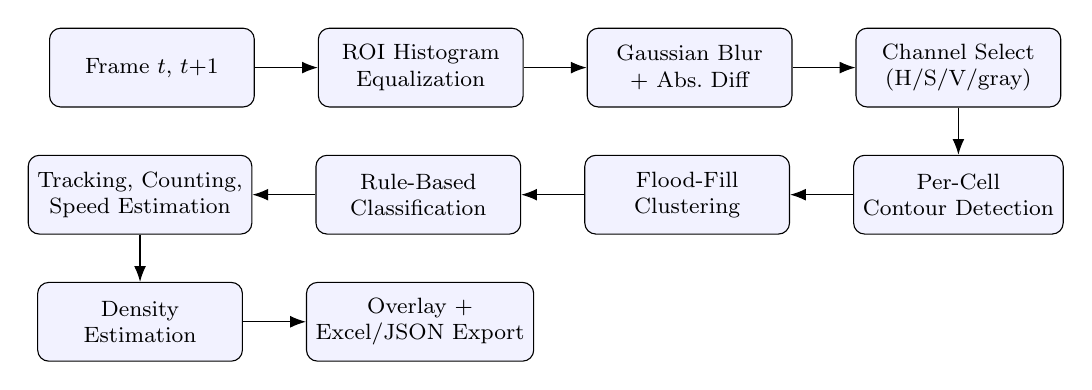
\begin{tikzpicture}[
  node distance=6mm and 8mm,
  box/.style={draw, rounded corners, align=center, minimum height=1.0cm,
              minimum width=2.6cm, font=\footnotesize, fill=blue!5},
  arr/.style={-{Latex[length=2mm]}}
]
\node[box] (frames) {Frame $t$, $t{+}1$};
\node[box, right=of frames] (he) {ROI Histogram\\Equalization};
\node[box, right=of he] (diff) {Gaussian Blur\\+ Abs.\ Diff};
\node[box, right=of diff] (chan) {Channel Select\\(H/S/V/gray)};
\node[box, below=of chan] (cell) {Per-Cell\\Contour Detection};
\node[box, left=of cell] (cluster) {Flood-Fill\\Clustering};
\node[box, left=of cluster] (classify) {Rule-Based\\Classification};
\node[box, left=of classify] (track) {Tracking, Counting,\\Speed Estimation};
\node[box, below=of track] (density) {Density\\Estimation};
\node[box, right=of density] (overlay) {Overlay +\\Excel/JSON Export};

\draw[arr] (frames) -- (he);
\draw[arr] (he) -- (diff);
\draw[arr] (diff) -- (chan);
\draw[arr] (chan) -- (cell);
\draw[arr] (cell) -- (cluster);
\draw[arr] (cluster) -- (classify);
\draw[arr] (classify) -- (track);
\draw[arr] (track) -- (density);
\draw[arr] (density) -- (overlay);
\end{tikzpicture}
\caption{Per-ROI processing pipeline shared by both implementations.
The sequential implementation runs one instance of this pipeline per
frame (ROI~1 only); the parallel implementation runs two instances per
frame (ROI~1 and ROI~2), dispatched as described in
Section~\ref{sec:parallel} and Fig.~\ref{fig:threadpools}.}
\label{fig:pipeline}
\end{figure*}

\subsection{Grid-Based Motion Detection}
\label{sec:motion}

This section's motion-detection front end is prior published work
\cite{baseline}, reused here as the input to the classification and
tracking layers of Sections~\ref{sec:cluster}--\ref{sec:tracking}. It is
described only to the depth needed to fix notation and to document two
adaptations made in the course of this work: the per-cell detection
thresholds were retuned (Section~\ref{sec:cellcontour}) because the
classification stage added here depends on precise contour geometry in
a way the baseline's simple occupancy check did not, and two latent
preprocessing bugs in the reused code were found and fixed
(Section~\ref{sec:crosscheck}).

\subsubsection{Contrast Normalization}
Before differencing, the pipeline applies histogram equalization
restricted to the ROI. The code implements two modes -- full grayscale
equalization of the ROI (\code{cv2.equalizeHist} applied after a
grayscale conversion), or equalization of a single HSV channel (H, S,
or V) with the other two channels left unmodified before converting
back to BGR -- but the equalization channel is hard-coded to V
(\code{he\_choice='V'}) independently of the \code{color\_channel}
setting, so only V-channel equalization is exercised in this paper. This
is applied independently to both input frames prior
to differencing, so that the differencing step operates on
contrast-normalized ROIs rather than raw pixel intensities, which
reduces sensitivity to slow lighting drift across the sequence.

\subsubsection{Frame Differencing and Channel Selection}
Both equalized frames are Gaussian-blurred ($7\times7$ kernel) and
absolute-differenced. The result is converted to HSV, and a
configurable subset of channels is split out (H, S, V, or any
combination, or plain grayscale via a separate \code{gray} code path).
This is a user-facing configuration knob (\code{color\_channel} in
\code{user\_input\_data.json}) that trades sensitivity to
illumination-only motion (grayscale/V) against sensitivity to
hue/saturation-varying motion (H/S), and directly determines how many
independent per-cell contour computations are required (one per
selected channel).

\subsubsection{Per-Cell Contour Detection}
\label{sec:cellcontour}
Each grid cell of each selected channel image is independently
Gaussian-blurred ($5\times5$), thresholded at a fixed intensity of 60,
and dilated with a rectangular structuring element sized to the cell
itself (\code{grid\_width} $\times$ \code{grid\_height}/2, 5 iterations)
to bridge small gaps in a vehicle's motion silhouette before contour
extraction via \code{cv2.findContours} (Suzuki--Abe border following
\cite{suzuki1985}). A contour is accepted only if its area exceeds 100
px$^2$. A cell is marked ``hot'' (binary result matrix entry $=1$)
\emph{only if every selected channel independently reports at least one
valid contour} -- an AND-across-channels rule intended to suppress
motion detected in only one channel (e.g., a shadow that perturbs V but
not H or S).

Relative to the baseline \cite{baseline}, this work retuned four of
these parameters -- the threshold intensity (20 $\to$ 60), the dilation
kernel (a fixed, cell-independent kernel with 3 iterations $\to$ a
cell-sized kernel with 5 iterations), the contour retrieval mode
(\code{RETR\_TREE} $\to$ \code{RETR\_EXTERNAL}), and the blur's sigma
(0 $\to$ 1) -- because Section~\ref{sec:classify}'s classifier depends
on a cluster's precise \code{col\_span}/\code{row\_span}, which is far
more sensitive to over- or under-dilated, nested, or noisy contours
than the baseline's simple presence/absence occupancy check ever was.
The minimum contour area (100 px$^2$) is unchanged from the baseline,
except that the comparison changed from $\geq$ to $>$.

\begin{table}[t]
\centering
\caption{Key pipeline parameters (identical in both implementations
unless noted).}
\label{tab:params}
\footnotesize
\begin{tabular}{p{3.6cm}p{3.9cm}}
\toprule
\textbf{Parameter} & \textbf{Value} \\
\midrule
ROI~1 (x, y, w, h) & (47, 202, 441, 141) \\
ROI~2 (x, y, w, h), parallel only & (500, 202, 441, 141) \\
Grid dimensions (rows $\times$ cols) & configurable, \code{user\_input\_data.json} \\
Cell blur / threshold & $5\times5$ Gaussian, $T{=}60$ \\
Cell dilation & (cell\_w, cell\_h/2) kernel, 5 iters \\
Min.\ contour area (cell) & 100 px$^2$ \\
Frame-diff blur & $7\times7$ Gaussian \\
Track match radius & ROI height / 2 \\
Duplicate-track IoU threshold & 0.40 \\
Crossing cooldown & 30 frames, 60 px \\
Label EWA $\alpha$ & 0.15 \\
Min.\ frames before label scored & 5 \\
Min.\ speed sample displacement & 3 $\times$ grid-cell height \\
Speed smoothing window & last 15 samples \\
Density blend weights & 0.7 (smoothed) / 0.3 (flow) \\
Density thresholds (first 50 samples) & 0.30 (Low/Med), 0.60 (Med/High) \\
Density base thresholds (adaptive) & 0.25 (Low/Med), 0.55 (Med/High) \\
Density threshold adaptation & $\pm$0.10, active after $>$50 samples \\
Flow normalization & 8 crossings per 2-s window \\
Track eviction & unseen for $>2\,$s ($2\times$FPS frames) \\
\code{\_CELL\_POOL} size (parallel) & $\min(32, 4\times\text{cpu\_count})$ (32 here) \\
\code{\_LANE\_POOL} size (parallel) & 2 \\
\bottomrule
\end{tabular}
\end{table}

\subsection{Spatial Clustering and Object Formation}
\label{sec:cluster}

The baseline implementation \cite{baseline} stops at the per-cell binary
occupancy grid of Section~\ref{sec:motion}; everything from this section
onward is this paper's contribution, starting with converting that
occupancy grid into discrete, per-vehicle candidate objects.

Hot cells are grouped into candidate vehicle objects by 4-connected
flood fill (\code{group\_cells}): starting from any unvisited hot cell,
a depth-first search over its row/column neighbors collects a maximal
connected component of hot cells, repeated until every hot cell belongs
to exactly one cluster. The current implementation note in the source
records that this flood-fill approach replaced an earlier
distance/column-based merge heuristic (retained, disabled, in the
source as \code{split\_cluster\_by\_columns}) because flood fill gives
geometrically accurate column-span and row-span values directly from
connectivity rather than from a heuristic distance threshold.

Each cluster is converted to an object (\code{cluster\_to\_object}) with
a bounding box derived from the pixel extents of its member cells, a
centroid at the bounding-box center, and \code{col\_span}/\code{row\_span}
counts (the number of \emph{distinct} columns/rows occupied) used
directly by the classification stage below.

\subsection{Rule-Based Vehicle Classification}
\label{sec:classify}

This classification layer has no counterpart in the baseline
\cite{baseline}, which only ever reports cell-level motion/no-motion.

Classification (\code{classify\_by\_grid}) is purely geometric: column
span and row span are each normalized by the grid's column/row count,
and a cluster is labeled \textbf{Bus} if its normalized column span
exceeds 0.75, or if both normalized spans exceed 0.55; labeled
\textbf{Van} if its normalized row span exceeds 0.45 (and it was not
already labeled Bus); and labeled \textbf{Car} otherwise. No appearance
or texture features are used -- classification is entirely a function
of how much of the calibrated grid a vehicle's motion silhouette
occupies. The source retains an earlier, continuous-score version of
this function (a weighted linear combination of the two normalized
spans against fixed cutoffs) commented out alongside the current
piecewise-conditional version, again indicating iterative tuning
against observed footprints rather than a principled decision boundary.
Because the thresholds are grid- and geometry-specific, this stage is
expected to be the least portable part of the pipeline across different
camera placements (see Section~\ref{sec:threats}).

\subsection{Tracking, Counting, and Speed Estimation}
\label{sec:tracking}

Per-vehicle identity tracking, line-crossing counting and implemented
speed estimation have no counterpart in the baseline \cite{baseline}
either (its paper counts vehicles from runs of occupied lattices and
leaves speed estimation to future work); this section (together with
Sections~\ref{sec:cluster} and \ref{sec:classify}) is the core
contribution this paper adds on top of it.

\subsubsection{Track Association}
Each frame's clustered objects are greedily matched to existing tracks
by nearest centroid, subject to a maximum distance of half the ROI
height and an exclusivity constraint (each existing track can absorb at
most one object per frame, enforced via a \code{matched\_track\_ids}
set). Unmatched objects spawn new tracks with a fresh integer ID; a track
not matched for more than $2\times$FPS frames (2\,s) is evicted.

\subsubsection{Temporal Label Smoothing}
Each track accumulates a raw per-frame classification from
Section~\ref{sec:classify} into a weighted-vote accumulator. The weight
combines a vertical-position term ($cy / \text{frame\_height}$, on the
premise that classifications made after more of the vehicle has entered
the ROI are more reliable) with an exponential temporal term
$(1+\alpha)^{\text{frame\_age}}$, $\alpha=0.15$, that up-weights more
mature tracks. The track's scored label (\code{final\_label}) is the
argmax of this accumulator. A separate, simpler mode vote over the last
10 raw labels (\code{display\_label}) drives the live on-screen overlay,
decoupled from the accumulator used for evaluation. A track's
classification is only accepted into the DETRAC evaluation once it has
survived at least \code{MIN\_FRAMES\_FOR\_LABEL}~$=5$ frames, filtering
early single-frame misclassifications before enough temporal evidence
has accumulated.

\subsubsection{Duplicate-Track Suppression}
\label{sec:dupsupp}
Within a frame, any two concurrently active tracks whose bounding boxes
overlap with IoU $>0.40$ are treated as duplicates of the same physical
vehicle; the younger track (by \code{age}, ties broken by the larger
numeric ID) is suppressed -- marked \code{counted} and evicted on the
next stale-track sweep -- so that a single vehicle that has momentarily
fragmented into two nearby clusters cannot register two crossings or
two classifications.

\subsubsection{Line-Crossing Counting}
A horizontal count line is fixed at the vertical midpoint of the ROI. A
track registers a crossing when its previous centroid was above the
line and its current centroid is at or below it, subject to a minimum
track age of 2 frames (to suppress spurious crossings from tracks
initialized directly on the line) and a cooldown filter
(\code{is\_duplicate\_crossing}): a crossing within 30 frames and 60 px
of a previously counted crossing is treated as a duplicate and
discounted, guarding against fragmented tracks re-triggering the count.

\subsubsection{Speed Estimation}
\label{sec:speed}
Displacement is accumulated from a reference centroid until it exceeds
\code{MIN\_SPEED\_DIST\_PX} $= 3\times$ grid-cell height -- large enough
to average out grid-quantization noise in the centroid position -- at
which point a speed sample (km/h) is computed from the accumulated pixel
displacement, the elapsed frame count, the video's FPS, and an
operator-supplied \code{pixels\_per\_meter} calibration constant, and
folded into a 15-sample rolling mean. \textbf{Implementation
inconsistency (found and fixed):} the parallel implementation guards
this computation on \code{self.pixels\_per\_meter > 0}, so speed
estimation is a no-op under an uncalibrated (zero) constant; the
sequential implementation originally performed the equivalent division
without this guard. Because the distance is a NumPy float, dividing by a
zero constant does not raise but yields \code{inf}, i.e.\ spurious
``inf km/h'' speeds whenever \code{pixels\_per\_meter} is left at its
default of 0 (\code{user\_input\_data.example.json}). The guard has been
added to \code{seq.py}; see Section~\ref{sec:threats}. \textbf{Speed
estimates are not validated in this paper}: no calibrated speed ground
truth exists for the benchmark sequences and the calibration constant is
0 in all benchmark runs, so speed estimation is inactive there.
Pixel-displacement speeds require an appropriate metric scale and
validation against measured speeds \cite{kamil2024}, and unstable
trajectories -- here, grid-quantized centroids -- degrade them
\cite{sangsuwan2024}.

\subsection{Adaptive Traffic Density Estimation}
\label{sec:density}

The baseline code \cite{baseline} computes and prints this same raw
occupancy fraction per frame (and, in its dual-ROI variant, per lane);
the baseline paper defines density from lattice-run vehicle counts per
unit area. Neither smooths it, blends it with flow, or thresholds it
into traffic-state labels -- that adaptive layer is added here.

Instantaneous density is the fraction of hot cells in the current
frame. It is smoothed with a rolling mean over approximately one second
of frames and blended (0.7/0.3) with a flow term -- the number of line
crossings in the last $2\times$FPS frames ($\approx$2\,s), divided by 8
and capped at 1, i.e.\ saturating at 8 crossings per 2-s window -- into a
single \code{combined\_density} score. For the first 50 samples fixed
thresholds of 0.30/0.60 are used. Once more than 50 combined-density
samples have accumulated, the Low/Medium/High classification thresholds
adapt: the 33rd and 66th percentiles of the density history are computed
and used to nudge the fixed base thresholds (0.25, 0.55) by at most
$\pm0.10$, preventing unbounded drift while allowing the system to
self-calibrate to the specific scene's typical occupancy range.

\subsection{Parallel Implementation}
\label{sec:parallel}

\subsubsection{Design Goals}
The baseline's \cite{baseline} preliminary dual-ROI implementation
already used a thread pool, but created it every frame and stored no
persistent per-lane tracking state -- adequate for a stateless per-frame
occupancy check. The tracking, label smoothing and speed estimation this
paper adds (Sections~\ref{sec:cluster}--\ref{sec:tracking}) need state
that persists across frames, per lane; the parallel implementation
described here therefore introduces \code{LaneTracker} instances that
hold it, together with persistent pools: it preserves
the algorithm and output semantics of Sections~\ref{sec:motion}--\ref{sec:density}
exactly, while restructuring execution to (i) support two independent
ROIs/lanes with persistent per-lane tracking state and (ii) exploit two
latent axes of parallelism: the rows$\times$cols largely-independent
per-cell contour computations within a single ROI, and the two
independent ROIs/lanes themselves.

\subsubsection{Persistent Thread-Pool Architecture}
\label{sec:pools}
Two long-lived \code{ThreadPoolExecutor} pools are created once at
module load, rather than once per frame (the overhead of the latter
approach -- repeated thread creation/teardown every frame -- is the
motivating problem this design fixes):

\begin{itemize}
\item \code{\_CELL\_POOL}, sized $\min(32,\,4\times\text{cpu\_count})$:
handles the fine-grained, GIL-releasing native work -- per-grid-cell
contour extraction (\code{LaneTracker.process\_grid\_cell}, dispatched
via \code{\_CELL\_POOL.map}) and per-ROI histogram equalization
(\code{apply\_histogram\_equalization\_parallel}, submitted by the main
thread via \code{\_CELL\_POOL.submit}, one task per ROI).
\item \code{\_LANE\_POOL}, sized 2: dispatches lane-level work -- each
lane's \code{process\_grid} call and each lane's
\code{compute\_tracking} call -- one \code{submit} per lane per stage.
\end{itemize}

The two pools are kept separate specifically because lane-level tasks
submitted to \code{\_LANE\_POOL} internally submit further work to
\code{\_CELL\_POOL}; if both stages shared one pool, a lane-level task
could occupy a worker slot while waiting on a nested submission to the
same pool, risking a self-nesting deadlock under worker-count
starvation. The full-frame preprocessing that follows equalization (the
$7\times7$ blur of both frames, \code{absdiff}, HSV conversion and channel
split) runs serially on the main thread and is shared by both lanes.
Fig.~\ref{fig:threadpools} illustrates the dispatch structure for one
frame.

\begin{figure}[t]
\centering
\resizebox{\columnwidth}{!}{%
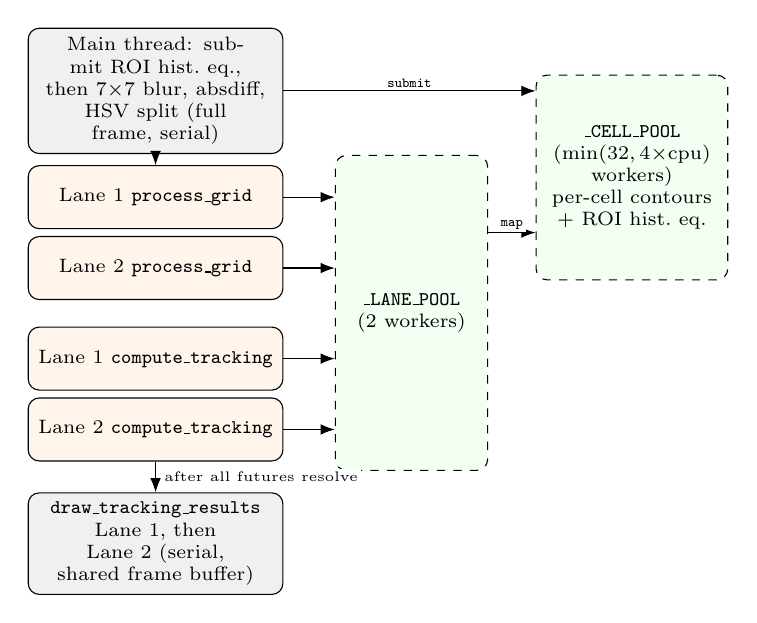
\begin{tikzpicture}[
  box/.style={draw, rounded corners, align=center, minimum height=0.8cm,
              text width=3.0cm, font=\scriptsize, fill=orange!8},
  serial/.style={box, fill=gray!12},
  pool/.style={draw, dashed, rounded corners, align=center, font=\scriptsize,
               fill=green!5, text width=1.7cm},
  arr/.style={-{Latex[length=1.8mm]}},
  lbl/.style={font=\tiny, fill=white, inner sep=1pt}
]
% main thread, top to bottom
\node[serial] (pre)   at (0, 0)    {Main thread: submit ROI hist.\ eq.,\\then $7{\times}7$ blur, absdiff,\\HSV split (full frame, serial)};
\node[box]    (l1)    at (0,-1.35) {Lane 1 \code{process\_grid}};
\node[box]    (l2)    at (0,-2.25) {Lane 2 \code{process\_grid}};
\node[box]    (t1)    at (0,-3.40) {Lane 1 \code{compute\_tracking}};
\node[box]    (t2)    at (0,-4.30) {Lane 2 \code{compute\_tracking}};
\node[serial] (draw)  at (0,-5.75) {\code{draw\_tracking\_results}\\Lane 1, then Lane 2 (serial,\\shared frame buffer)};
% pools
\node[pool, minimum height=4.0cm] (lanepool) at (3.25,-2.82) {\code{\_LANE\_POOL}\\(2 workers)};
\node[pool, minimum height=2.6cm, text width=2.2cm] (cellpool) at (6.05,-1.10) {\code{\_CELL\_POOL}\\($\min(32,4{\times}\text{cpu})$\\workers)\\per-cell contours\\+ ROI hist.\ eq.};
% arrows: lane-level submissions (horizontal, no crossings)
\foreach \n in {l1,l2,t1,t2} \draw[arr] (\n.east) -- (\n.east -| lanepool.west);
% histogram equalization: main thread -> cell pool
\draw[arr] (pre.east) -- node[lbl, above]{\code{submit}} (pre.east -| cellpool.west);
% per-cell fan-out from process_grid tasks
\draw[arr] (lanepool.east |- l1.east) ++(0,-0.45) coordinate (a) -- node[lbl, above]{\code{map}} (a -| cellpool.west);
% ordering
\draw[arr] (pre.south) -- (l1.north);
\draw[arr] (t2.south) -- node[lbl, right, xshift=2pt]{after all futures resolve} (draw.north);
\end{tikzpicture}%
}
\caption{Per-frame dispatch structure. The main thread submits the
per-ROI histogram equalization to \code{\_CELL\_POOL}, then performs the
full-frame blur/difference/channel split serially. Grid detection and
tracking-state updates for both lanes are submitted to
\code{\_LANE\_POOL}; each lane's grid detection fans out per-cell work
to \code{\_CELL\_POOL}. Only \code{draw\_tracking\_results} touches the
shared frame buffer, and it is called serially for both lanes after both
lanes' state updates have completed.}
\label{fig:threadpools}
\end{figure}

\subsubsection{Per-Lane State Encapsulation}
The sequential implementation keeps all mutable state -- track
dictionary, next track ID, vehicle count, crossing history, density
history, per-frame evaluation snapshots -- as module-level globals. The
parallel implementation moves all of this into a \code{LaneTracker}
class, instantiated once per lane (\code{lane1}, \code{lane2}). This is
what makes concurrent per-lane execution safe: each lane's
\code{compute\_tracking} call reads and writes only that instance's own
attributes, so two lanes' calls submitted to \code{\_LANE\_POOL} touch
disjoint memory and cannot race with each other.

\subsubsection{Concurrency Safety: Compute/Draw Separation}
The one piece of state that \emph{is} shared between lanes is the frame
buffer itself (\code{frame1}), which both lanes annotate with grid
overlays, bounding boxes, and HUD text. \code{LaneTracker} splits its
per-frame update into \code{compute\_tracking} (pure state
bookkeeping -- track association, label accumulation, counting; no
drawing) and \code{draw\_tracking\_results} (all \code{cv2} drawing
calls onto \code{frame1}; no state mutation). \code{compute\_tracking}
for both lanes is dispatched concurrently via \code{\_LANE\_POOL};
\code{draw\_tracking\_results} is then called serially, lane 1 then
lane 2, only after both futures have resolved. This ordering guarantee
-- rather than any lock -- is what prevents interleaved drawing calls
from producing an inconsistent overlay on the shared array, and it holds
regardless of whether the GIL would additionally serialize the
underlying array writes.

It is worth stating plainly what this design does \emph{not} claim:
\code{compute\_tracking} is overwhelmingly pure-Python dictionary and
list bookkeeping, not GIL-releasing numeric work over large arrays, so
running the two lanes' \code{compute\_tracking} calls in separate
threads is not expected to yield a proportional wall-clock speedup the
way the \code{\_CELL\_POOL}-dispatched OpenCV stage is. The
architectural benefit of the compute/draw split is safety and clarity --
a race-free separation of ``update state'' from ``touch the shared
frame'' -- not a guaranteed CPU-bound speedup in that stage. This
prediction is tested directly in Section~\ref{sec:results} against
per-stage \code{cProfile} timings.

\subsubsection{Expected Sources and Limits of Speedup}
\label{sec:speedup-limits}
CPython's GIL serializes execution of Python bytecode across threads
within one process \cite{pythongil}; a thread pool therefore yields
genuine parallel speedup specifically for the fraction of the workload
spent inside GIL-releasing native calls. In this pipeline that fraction
is expected to be large for the \code{\_CELL\_POOL}-dispatched stage
(\code{GaussianBlur}, \code{threshold}, \code{dilate},
\code{findContours}, and \code{equalizeHist} are all compiled OpenCV
routines) and small for the pure-Python tracking/bookkeeping stage
inside \code{compute\_tracking}. Under Amdahl's law
(Eq.~\eqref{eq:amdahl}), the pipeline's overall achievable speedup is
therefore bounded above by the fraction of total per-frame time spent in
the GIL-releasing stage, not by worker count alone -- a bound this paper
measures directly rather than assumes (Section~\ref{sec:results}). A
further limit applies if the native calls are themselves already
multithreaded: Python-level threads then compete for cores that are
already busy, and the ceiling of Eq.~\eqref{eq:amdahl} is not reached
(Section~\ref{sec:why}).

\subsection{Ground-Truth Evaluation Methodology}
\label{sec:eval}

Both implementations evaluate against UA-DETRAC XML ground truth
\cite{wen2020} using identical logic (procedural in \code{seq.py};
parameterized per-lane in \code{rparallel\_he3.py}'s
\code{evaluate\_lane}), so the evaluation methodology itself is not a
confound between the two implementations.

\subsubsection{Ground-Truth Parsing and Filtering}
Per-frame target lists are parsed from the DETRAC XML
(\code{load\_detrac}), each target's \code{vehicle\_type} attribute
mapped to \{Car, Van, Bus, Unknown\}, and ground-truth boxes are
restricted to those overlapping the relevant ROI
(\code{filter\_gt\_boxes\_to\_roi}) before any comparison is made.

\subsubsection{Grid-Level Evaluation}
For each frame, a ground-truth label grid is built by mapping each
in-ROI ground-truth box's center into a grid cell
(\code{create\_gt\_label\_grid}) and is compared cell-by-cell against
the pipeline's predicted label grid (Section~\ref{sec:tracking}), giving
a $4\times4$ confusion matrix over \{Empty, Car, Van, Bus\}.

\subsubsection{Vehicle-Level (ID-Based) Evaluation}
Independently of the grid, each predicted track with a scored label
(age $\geq$ \code{MIN\_FRAMES\_FOR\_LABEL}) is matched to the
highest-IoU ground-truth box in its frame (\code{match\_vehicle},
minimum IoU 0.1); the majority-voted predicted label across all frames
in which a given ground-truth ID was matched populates a
$3\times3$ Car/Van/Bus confusion matrix, from which per-class precision,
recall, and F1 are computed with a small epsilon (Eq.~\eqref{eq:f1}) to
avoid division by zero for unseen classes:
\begin{equation}
P = \frac{TP}{TP+FP+\epsilon},\qquad
R = \frac{TP}{TP+FN+\epsilon},
\label{eq:f1}
\end{equation}
\begin{equation}
F1 = \frac{2PR}{P+R+\epsilon}.
\label{eq:f1b}
\end{equation}
Separately, and independent of classification accuracy, a
grid-independent count is reported: the number of unique in-ROI
ground-truth IDs versus the number of unique predicted track IDs, with
matched/unmatched breakdowns on both sides -- separating \emph{counting}
performance from \emph{classification} performance. Four implementation
details affect absolute accuracy (identically in both implementations):
predictions for frame $t$ are compared with the ground truth of frame
$t{+}1$; a matched ground-truth vehicle of DETRAC type ``others'' is
scored as Car; DETRAC ignored regions are not masked; and track-to-box
matching is greedy per track, without a one-to-one constraint.

\section{Experimental Setup}
\label{sec:experiments}

\subsection{Hardware, Software, and Data}
\begin{itemize}
\item CPU: AMD Ryzen 5 7235HS, 4 cores / 8 logical processors (laptop);
\code{\_CELL\_POOL} therefore has $\min(32, 4\times8)=32$ workers
\item OS: Windows 11 (build 26300)
\item Python 3.12.3 (CPython); OpenCV 4.12.0; NumPy 1.26.4
\item Dataset: UA-DETRAC, 12 sequences selected across the four weather
categories (Section~\ref{sec:selection-detail}); all 12 are
$960\times540$ at 25\,fps
\item Grid dimensions: $6\times6$; \code{color\_channel}: V
\item \code{pixels\_per\_meter}: 0 (uncalibrated for these sequences --
speed estimation inactive, per Section~\ref{sec:speed})
\item GUI display and per-frame JPEG dump disabled for all benchmark runs
(\code{BTP\_DISPLAY=0}, \code{BTP\_SAVE\_FRAMES=0})
\item Repeated runs per video: 1 per workload (see
Section~\ref{sec:threats})
\end{itemize}
Every metrics file records the platform, CPU model, physical and logical
core counts and the Python/OpenCV/NumPy versions, following the
reporting recommendations of \cite{beyer2019}.

\subsection{Video Selection}
\label{sec:selection-detail}
Twelve videos were selected from the UA-DETRAC Cloudy/Night/Rainy/Sunny
folders using an orchestration script that (i) computed a traffic-density
proxy (mean annotated vehicles per frame) directly from each candidate's
DETRAC XML ground truth, (ii) split each category's videos into
light/medium/heavy terciles by that density, and (iii) selected the
middle-ranked video of each tercile (the upper of the two middle videos
when a tercile has an even count), balanced across all four categories
(3 tiers $\times$ 4 categories = 12). The candidate pools were small and
uneven (Cloudy 4, Night 6, Rainy 5, Sunny 23 videos with annotations),
and the tiers are \emph{relative within each category}: the Sunny
``light'' video (6.73) is denser than the Cloudy ``heavy'' video (6.40).
All 12 selected videos had a matching XML annotation (0 missing).
Selected sequences and their measured density (mean GT vehicles/frame)
were: Cloudy -- MVI\_39761 (2.81, light), MVI\_39771 (6.32, medium),
MVI\_40963 (6.40, heavy); Night -- MVI\_40774 (6.09, light), MVI\_40773
(8.03, medium), MVI\_40772 (12.93, heavy); Rainy -- MVI\_63525 (3.52,
light), MVI\_40141 (3.89, medium), MVI\_40131 (9.32, heavy); Sunny --
MVI\_20033 (6.73, light), MVI\_20011 (11.53, medium), MVI\_39311 (14.92,
heavy). Processed frame pairs per video (video length $-1$) were, in the
same order: 1659, 569, 1819; 949, 984, 1199; 984, 1599, 1644; 783, 663,
1504 (14{,}356 in total).

\subsection{Fair-Comparison Protocol}
\label{sec:fair}
The two implementations as shipped are \emph{not} directly comparable
by raw wall-clock time: \code{seq.py} processes one ROI per frame,
while \code{rparallel\_he3.py} processes two. We therefore time four
workloads per video, all with identical videos, ROIs, grid,
preprocessing and evaluation settings:
\begin{center}
\footnotesize
\setlength{\tabcolsep}{4pt}
\begin{tabular}{lllc}
\toprule
\textbf{ID} & \textbf{Script} & \textbf{Setting} & \textbf{Lanes} \\
\midrule
A & \code{seq.py} & -- & 1 \\
B & \code{rparallel\_he3.py} & \code{BTP\_LANES=1}, threaded & 1 \\
C & \code{rparallel\_he3.py} & \code{BTP\_EXECUTOR=serial} & 2 \\
D & \code{rparallel\_he3.py} & default, threaded & 2 \\
\bottomrule
\end{tabular}
\end{center}
In C, both thread pools are replaced by an inline executor that runs each
submitted task immediately on the main thread: the same
\code{LaneTracker} code, ROIs and call order as D, without threads. With
$T$ the end-to-end wall time (video open, writer setup and all frames)
and $\bar t$ the mean of the per-frame timer (Section~\ref{sec:instr}),
we report, per video:
\begin{itemize}
\item $S_{\text{naive}} = T_A/T_D$ -- raw ratio, workload-confounded,
context only;
\item $S_{\text{norm}} = \Theta_D/\Theta_A = 2\,T_A/T_D$, with ROI-frame
throughput $\Theta = (\text{frames}\times\text{lanes})/T$ -- a throughput
ratio, not an execution-time speedup; its per-frame-loop form is
$S_{\text{norm,pf}} = 2\,\bar t_A/\bar t_D$;
\item $S_{\text{amort}} = 2\,T_A/T_C$ -- the same normalization for the
\emph{unthreaded} two-lane run, i.e.\ the gain from processing two lanes
per decoded frame without any threading;
\item $S_{\text{same}} = T_C/T_D$ (two lanes) and $T_A/T_B$ (one lane)
-- same workload with and without threads, isolating the effect of
threading.
\end{itemize}
Because decoding, video writing and the full-frame
blur/difference/channel split are done once per frame regardless of lane
count, $S_{\text{norm}}$ can exceed 1 through this sharing alone; it must
not be read as a threading speedup without $S_{\text{same}}$. All figures
are computed per video by \code{benchmarking/orchestrate\_benchmark.py}
and summarized as mean $\pm$ sample standard deviation over the 12 videos;
this spread is between-video variation, not repeated-run uncertainty.
Parallel efficiency is $E(N)=S_{\text{same}}/N$ for $N=2$
(\code{\_LANE\_POOL} width), $N=4$ (physical cores) and $N=8$ (logical
processors), and $S_{\text{same}}$ is compared with the Amdahl ceiling of
Eq.~\eqref{eq:amdahl} using $p$ estimated from \code{cProfile} output
(Section~\ref{sec:results-amdahl}).

\subsection{Instrumentation}
\label{sec:instr}
Each run exports end-to-end wall time; per-frame processing time
(\code{frame\_times\_seconds}), which covers preprocessing, per-cell
detection, clustering, classification, tracking/counting/speed, density
and all overlay drawing and stops before output I/O, with identical
boundaries in both scripts; per-frame output I/O time (video write,
preview, decoding the next frame); per-frame resident memory; process CPU
time; the system record above; and, with DETRAC ground truth, the
grid-level and vehicle-level confusion matrices and per-class
precision/recall/F1 of Section~\ref{sec:eval}. Each video is run with a
clean pass (profiler off) for every workload, used for all timing, and a
profiled pass (\code{cProfile}) for workloads A and D, used only for
Section~\ref{sec:results-amdahl}.

\textbf{Timing artifact (found and fixed).}\label{sec:timingfix} In an
earlier measurement round the sequential script polled
\code{cv2.waitKey} twice per frame and wrote a JPEG of every frame, while
neither cost was paired in the parallel script; with these unconditional,
the sequential run was inflated and an earlier, unarchived wall-clock
comparison suggested a speedup of roughly $3.3\times$. Both are now gated
on the display/save switches. The surviving pre-fix profiles (different
videos, $10\times10$ grid) show \code{waitKey} at 43.0\,s and
\code{imwrite} at 7.6\,s of an 83.5\,s run; the $3.3\times$ figure itself
could not be recovered and is not used anywhere in this paper.

\textbf{Earlier benchmark run.} A first run of workloads A and D on the
same machine and videos used instrumented copies of the scripts whose
per-frame timers had different boundaries (the sequential timer stopped
before the video write, the parallel one after it) and which did not
record sequential memory. It gave $S_{\text{naive}}=0.631\pm0.042$,
$S_{\text{norm}}=1.261\pm0.084$ and $S_{\text{norm,pf}}=1.079\pm0.064$,
and per-video F1 scores identical to those reported below. All results
in Section~\ref{sec:results} are from the re-run of the shipped scripts
with the corrected instrumentation.

\section{Results and Discussion}
\label{sec:results}

Results are from the 12-video benchmark described in
Section~\ref{sec:selection-detail}, run with the shipped, corrected
scripts (Section~\ref{sec:crosscheck}).

\subsection{Accuracy: Verified Equivalence}
Across all 12 videos, \code{seq.py} and the parallel implementation's
Lane~1 produced matching Car/Van/Bus F1 scores and confusion matrices
(compared exactly, on every class and video), and the earlier benchmark
run gave the same per-video values. Table~\ref{tab:accuracy-by-cat}
therefore reports a single accuracy figure per category (identical
between implementations); per-tier figures are in
Table~\ref{tab:accuracy-by-tier}.

\begin{table}[t]
\centering
\caption{Classification F1 by weather category, mean $\pm$ std over 3
videos/category (identical between \code{seq.py} and parallel Lane~1;
Section~\ref{sec:crosscheck}).}
\label{tab:accuracy-by-cat}
\footnotesize
\begin{tabular}{lccc}
\toprule
\textbf{Category} & \textbf{Car F1} & \textbf{Van F1} & \textbf{Bus F1} \\
\midrule
Cloudy & $0.281 \pm 0.292$ & $0.054 \pm 0.094$ & $0.133 \pm 0.231$ \\
Night  & $0.396 \pm 0.400$ & $0.000 \pm 0.000$ & $0.000 \pm 0.000$ \\
Rainy  & $0.181 \pm 0.158$ & $0.210 \pm 0.101$ & $0.042 \pm 0.072$ \\
Sunny  & $0.283 \pm 0.490$ & $0.167 \pm 0.289$ & $0.000 \pm 0.000$ \\
\bottomrule
\end{tabular}
\end{table}

\begin{table}[t]
\centering
\caption{Classification F1 by traffic-density tier, mean $\pm$ std over
4 videos/tier.}
\label{tab:accuracy-by-tier}
\footnotesize
\begin{tabular}{lccc}
\toprule
\textbf{Tier} & \textbf{Car F1} & \textbf{Van F1} & \textbf{Bus F1} \\
\midrule
Light  & $0.065 \pm 0.130$ & $0.187 \pm 0.239$ & $0.000 \pm 0.000$ \\
Medium & $0.408 \pm 0.354$ & $0.071 \pm 0.143$ & $0.000 \pm 0.000$ \\
Heavy  & $0.382 \pm 0.352$ & $0.064 \pm 0.079$ & $0.131 \pm 0.189$ \\
\bottomrule
\end{tabular}
\end{table}

The high standard deviations relative to the means (e.g.\ Sunny Car F1
$0.283 \pm 0.490$) reflect the small per-cell sample size (3--4 videos)
combined with genuinely bimodal per-video outcomes -- several videos
score 0 on a class because that class was absent or never reached
\code{MIN\_FRAMES\_FOR\_LABEL} age in that particular ROI/video, not
because of graded misclassification. Bus F1 is 0 for Night, Sunny, and
the light/medium density tiers entirely -- consistent with
Section~\ref{sec:classify}'s expectation that the geometric classifier's
fixed span thresholds are the least portable part of the pipeline.
These absolute accuracies are low; the contribution of this section is
the verified agreement between implementations, not the classifier's
accuracy.

\subsection{Timing: Four Workloads}
\label{sec:timing}
Table~\ref{tab:results-timing} reports the clean-pass timing of the four
workloads.

\begin{table}[t]
\centering
\caption{Timing of the four workloads (clean pass), mean $\pm$ std over
12 videos (between-video variation).}
\label{tab:results-timing}
\scriptsize
\setlength{\tabcolsep}{2.5pt}
\begin{tabular}{lcccccc}
\toprule
 & \textbf{Ln.} & \textbf{Loop$^{a}$} & \textbf{I/O$^{a}$} & \textbf{FPS$^{b}$} & \textbf{Peak} & \textbf{CPU$^{c}$} \\
 & & (ms) & (ms) & & (MB) & (cores) \\
\midrule
A & 1 & $9.41\pm1.84$ & $2.26\pm0.46$ & $81.1\pm15.7$ & $302.5\pm1.9$ & $4.20\pm0.61$ \\
B & 1 & $11.10\pm1.99$ & $2.19\pm0.43$ & $72.0\pm12.2$ & $306.4\pm1.8$ & $4.01\pm0.50$ \\
C & 2 & $14.54\pm2.59$ & $2.09\pm0.36$ & $58.2\pm9.6$ & $306.0\pm3.0$ & $4.52\pm0.47$ \\
D & 2 & $17.46\pm3.73$ & $2.27\pm0.39$ & $50.1\pm9.4$ & $310.0\pm3.1$ & $3.94\pm0.70$ \\
\bottomrule
\end{tabular}

\smallskip
\parbox{\columnwidth}{\scriptsize $^{a}$Per-frame processing incl.\ drawing
(Loop) and output I/O incl.\ next-frame decode (I/O); identical
boundaries in all workloads.
$^{b}$Video frames per second of end-to-end wall time.
$^{c}$Process CPU time divided by wall time.}
\end{table}

Per video, then averaged ($n=12$):
\begin{align}
S_{\text{naive}} &= T_A/T_D = 0.628 \pm 0.114,\\
S_{\text{norm}} &= 2\,T_A/T_D = 1.257 \pm 0.228,
\label{eq:measured-speedup}\\
S_{\text{norm,pf}} &= 2\,\bar t_A/\bar t_D = 1.097 \pm 0.187,\\
S_{\text{amort}} &= 2\,T_A/T_C = 1.458 \pm 0.216,\\
S_{\text{same}}^{(2)} &= T_C/T_D = 0.860 \pm 0.077,\\
S_{\text{same}}^{(1)} &= T_A/T_B = 0.900 \pm 0.123.
\end{align}
The per-frame-loop forms of the last two are $0.842\pm0.081$ and
$0.852\pm0.107$. Three findings follow. (i) The threaded two-lane run
takes longer than the one-lane sequential run on every video
($S_{\text{naive}}$ 0.43--0.85). (ii) \textbf{Threading does not reduce
execution time on this machine}: for the same two-lane workload, the
threaded run (D) is slower than the unthreaded run (C) on all 12 videos
($S_{\text{same}}^{(2)}$ 0.69--0.93), and the one-lane threaded run (B)
is slower than \code{seq.py} on 9 of 12 videos. (iii) The
workload-normalized throughput gain of D over A ($S_{\text{norm}}=1.26$,
above 1 on 10 of 12 videos) is \emph{smaller} than that of the
unthreaded two-lane run C over A ($S_{\text{amort}}=1.46$); it therefore
comes from processing two lanes per decoded and preprocessed frame, not
from threading. The parallel efficiency of the threads-only comparison
is $E(2)=0.43$, $E(4)=0.22$ and $E(8)=0.11$. Peak memory of the threaded
two-lane run is $7.5$\,MB (2.5\%) above \code{seq.py}.

\begin{table}[t]
\centering
\caption{Normalized throughput ($S_{\text{norm}}=2T_A/T_D$) and
threads-only ratio ($S_{\text{same}}^{(2)}=T_C/T_D$) by category and
density tier, mean $\pm$ std.}
\label{tab:speedup-breakdown}
\footnotesize
\begin{tabular}{lcc}
\toprule
\textbf{Group} & $S_{\text{norm}}$ & $S_{\text{same}}^{(2)}$ \\
\midrule
Cloudy & $1.329 \pm 0.323$ & $0.910 \pm 0.020$ \\
Night  & $1.316 \pm 0.146$ & $0.863 \pm 0.049$ \\
Rainy  & $1.220 \pm 0.241$ & $0.831 \pm 0.124$ \\
Sunny  & $1.162 \pm 0.269$ & $0.837 \pm 0.090$ \\
\midrule
Light  & $1.342 \pm 0.188$ & $0.889 \pm 0.037$ \\
Medium & $1.349 \pm 0.228$ & $0.874 \pm 0.027$ \\
Heavy  & $1.078 \pm 0.197$ & $0.818 \pm 0.126$ \\
\bottomrule
\end{tabular}
\end{table}

Table~\ref{tab:speedup-breakdown} breaks both ratios down by category and
density tier. Normalized throughput is lowest for the heavy tier, but the
tiers are ranked within each weather category rather than on an
absolute density scale (Section~\ref{sec:selection-detail}). Across the
12 videos, $S_{\text{norm}}$ correlates weakly and negatively with
measured density (Pearson $r=-0.45$; $-0.46$ in the earlier run). With
$n=12$ this is an observation, not an established effect, and the
profiles do not support a density-dependent, unparallelized tracking
stage as its cause: \code{process\_tracking\_counting} accounts for only
1.6--4.2\% of sequential run time on every video, with no trend in
density (2.8\% on the lightest video, 3.0\% on the densest), and
sequential loop time does not increase with density tier (light 11.4,
medium 8.4, heavy 8.4\,ms). The cause of the variation is undetermined.
Category-level variation is comparatively small and shows no clean
ordering by weather condition.

\subsection{Per-Stage Profiling and the Amdahl Ceiling}
\label{sec:results-amdahl}
The sequential implementation's \code{cProfile} breakdown for one video
(profiled pass, MVI\_39311, the densest of the twelve, 1504 frames,
18.62\,s profiled wall time) attributes self-time as follows: the seven
largest native OpenCV calls (\code{dilate}, \code{GaussianBlur},
\code{VideoCapture.read}, \code{cvtColor}, \code{absdiff},
\code{VideoWriter.write}, \code{split}) account for \textbf{12.40\,s
(66.6\% of total)}; Python-level wrapper/bookkeeping functions
(\code{process\_grid}, \code{process\_grid\_channel}, \code{process\_hsv},
\code{apply\_histogram\_equalization}, \code{density\_calculation},
\code{process\_tracking\_counting}, \code{numpy.percentile}) for 0.99\,s;
and \code{main}'s own loop overhead for 1.62\,s. The remaining 3.61\,s
consists of other native calls in the top-15 list (\code{findContours}
0.51\,s, \code{putText} 0.42\,s, \code{numpy.asanyarray} 0.30\,s,
\code{getStructuringElement} 0.26\,s, \code{rectangle} 0.25\,s,
\code{threshold} 0.20\,s; 1.95\,s together) and $\approx$1.66\,s in
functions below the top-15 cutoff (e.g.\ \code{group\_cells},
\code{cluster\_to\_object}, \code{classify\_by\_grid}).

Treating the seven largest native calls as parallelizable is optimistic:
\code{VideoCapture.read} and \code{VideoWriter.write} happen once per
frame regardless of lane count and are never dispatched to either thread
pool. Restricting to time reachable through \code{\_CELL\_POOL} (the
per-cell contour path inside \code{process\_grid\_channel}, plus
\code{apply\_histogram\_equalization}) gives $p_{\text{cellpool}} =
6.74\text{s}/18.62\text{s} = 0.362$. Over the profiled passes of all 12
videos, $p_{\text{cellpool}} = 0.375\pm0.019$ (range 0.349--0.400) and
the broad estimate is $0.667\pm0.011$. Table~\ref{tab:amdahl} lists the
resulting ceilings.

\begin{table}[t]
\centering
\caption{Amdahl's-law ceilings (Eq.~\eqref{eq:amdahl}) from the
MVI\_39311 profile vs.\ the measured threads-only ratio. $N{=}8$: logical
processors; $N{=}4$: physical cores; $N{=}2$: \code{\_LANE\_POOL} width.}
\label{tab:amdahl}
\footnotesize
\setlength{\tabcolsep}{4pt}
\begin{tabular}{lccccc}
\toprule
\textbf{Estimate of $p$} & \textbf{$p$} & \textbf{$S(\infty)$} & \textbf{$S(8)$} & \textbf{$S(4)$} & \textbf{$S(2)$} \\
\midrule
Broad (7 native calls) & 0.666 & 3.00 & 2.40 & 2.00 & 1.50 \\
Narrow (\code{\_CELL\_POOL}) & 0.362 & 1.57 & 1.46 & 1.37 & 1.22 \\
\midrule
\multicolumn{3}{l}{Measured $S_{\text{same}}^{(2)}=T_C/T_D$} & \multicolumn{3}{r}{$0.860 \pm 0.077$} \\
\multicolumn{3}{l}{Measured, per-frame loop} & \multicolumn{3}{r}{$0.842 \pm 0.081$} \\
\bottomrule
\end{tabular}
\end{table}

The measured threads-only ratio is below 1 and far below both ceilings,
even the narrow one at $N=2$ (1.22). An earlier draft of this analysis
compared the narrow ceiling with $S_{\text{norm}}$ and found close
agreement (1.24 vs.\ 1.26); the same-workload measurement shows that
agreement was coincidental, since $S_{\text{norm}}$ reflects shared
per-frame work rather than threading. Eq.~\eqref{eq:amdahl} assumes that
the parallel fraction runs on otherwise idle workers with no dispatch
cost; Section~\ref{sec:why} discusses why neither holds here, and the
single-fraction model cannot represent such contention
\cite{poolla2023}.

\subsection{Cross-Implementation Accuracy Check: Two Found and Fixed Divergences}
\label{sec:crosscheck}
Section~\ref{sec:overview}'s footnote already previews this, but it is
significant enough to document as a discussion point in its own right,
including the fact that it took two rounds to fully resolve. Because
\code{seq.py} and the parallel implementation's Lane~1 process the same
ROI on the same video with (supposedly) identical deterministic logic,
their per-video DETRAC confusion matrices should match exactly -- any
discrepancy indicates a bug rather than a legitimate
parallelism/accuracy trade-off. Running this check across the 12-video
benchmark (Section~\ref{sec:experiments}) found that only 4 of 12 videos
produced matching Car/Van/Bus F1 between the two implementations (the
pre-fix runs were not archived; the 4/12 and 5/12 match rates below are
from our working notes).

\textbf{First fix: missing pre-diff blur.} \code{seq.py}'s
\code{process\_hsv}/\code{process\_grayscale} apply a $7\times7$
Gaussian blur to both frames \emph{after} histogram equalization and
\emph{before} differencing; the parallel implementation's equivalent
functions differenced the equalized frames directly, with no such blur.
This was added to the parallel implementation, matching \code{seq.py}'s
kernel and sigma exactly.

\textbf{This alone was insufficient}: re-running the check afterward
improved the match rate only from 4/12 to 5/12, indicating a second,
independent divergence. Tracing it found a materially larger gap in the
same preprocessing stage: \textbf{the histogram equalization method
itself.} \code{seq.py} (with \code{he\_choice='V'}, hardcoded
independently of the \code{color\_channel} config used for diff-channel
selection) equalizes only the V channel in HSV space, leaving hue and
saturation untouched. The parallel implementation's
\code{apply\_histogram\_equalization\_single} had no
\code{channel\_choice} parameter at all and unconditionally converted
the ROI to grayscale before equalizing -- discarding all hue/saturation
information before the frame ever reached the differencing step. This
is a substantially larger change to the input than the missing blur:
it alters what information is available to every downstream stage, not
just its noise profile. A \code{channel\_choice}-aware version of this
function, branching identically to \code{seq.py}'s
\code{apply\_histogram\_equalization}, was added to the parallel
implementation, hardcoded to \code{'V'} to match \code{seq.py}'s current
(also hardcoded) behavior exactly. \code{seq.py} itself was not modified
by either fix.

Both fixes together are, to the best of our current code-level analysis,
the complete set: the per-cell contour-detection parameters (blur
kernel, threshold, dilation kernel and iteration count, minimum contour
area) and the track-matching radius were separately verified identical
between the two implementations' original source (not just the bench
copies), so the preprocessing stage was the sole remaining candidate for
a systematic divergence.

This two-round discovery is itself the methodological point worth
making: \textbf{two implementations described as ``the same algorithm,
just parallelized'' are an empirical claim, not a documentation claim,
and should be tested as one} -- and a single passing check (as the blur
fix alone appeared to be, improving the match rate) is not sufficient
evidence of full equivalence on its own; the match rate itself, not just
its direction of improvement, has to be verified. A wall-clock speedup
number computed between two implementations that are silently
processing different inputs is not measuring parallelization at all.

This was re-run after both fixes: \textbf{all 12 videos now produce
matching \code{seq.py} vs.\ parallel-Lane-1 confusion matrices} (vehicle
and grid level, ID-count summary and per-class precision, recall and F1
compared exactly), in both the clean and the profiled pass. The same
check covers the two additional workloads of Section~\ref{sec:fair}:
Lane~1 of the one-lane threaded run and of the two-lane unthreaded run
matches \code{seq.py} on all 12 videos, and Lane~2 matches between the
unthreaded and threaded two-lane runs, which also shows that adding
Lane~2 does not perturb Lane~1. On the benchmark machine all 60 checks
(12 videos $\times$ 5) were identical; the same 48 clean-pass checks were
also identical in a separate Linux environment with OpenCV~5.0. These
are checks on the 12 tested videos under this evaluation protocol, not a
proof of equivalence for every input; \code{orchestrate\_benchmark.py}
repeats them on every run.

\subsection{Why Threading Does Not Help Here}
\label{sec:why}
Three properties of this pipeline plausibly explain the result; only the
first is measured directly. (i) \textbf{The cores are already busy.}
\code{seq.py} runs a single Python thread, yet its process CPU time is
$4.20\pm0.61$ times its wall time (Table~\ref{tab:results-timing}): native
code inside OpenCV is already multithreaded within individual calls, so
the threads-only experiment adds Python-level threads on top of a
machine whose four physical cores are largely occupied. CPU time per
wall second does not rise with threading (3.94 cores for D vs.\ 4.52 for
C). (ii) \textbf{The dispatched tasks are small.} Each frame dispatches
36 per-cell tasks per lane, each a few native calls on a $73\times23$-pixel
cell (e.g.\ \code{dilate} averages $\approx$64\,$\mu$s per call in the
profile), so task submission, scheduling and result collection are a
significant fraction of each task. (iii) \textbf{The GIL serializes
everything else}: the Python wrappers, clustering, classification and
tracking (Section~\ref{sec:speedup-limits}). Separating (ii) and (iii)
would require experiments not done here, e.g.\ limiting OpenCV's internal
threads or batching cells per task. The baseline paper reports a 26.55\%
efficiency improvement for its parallel mode \cite{baseline}; its code,
configuration, measured quantity and hardware differ from ours, so our
results neither reproduce nor contradict that figure.

\subsection{Threats to Validity and Limitations}
\label{sec:threats}

\textbf{Single hand-tuned scene.} ROI coordinates and every threshold in
Table~\ref{tab:params} (blur kernels, the intensity threshold of 60 and
the 100\,px$^2$ area threshold, the 0.75/0.55/0.45 classification
breakpoints) were tuned for one camera geometry and are unlikely to
generalize to a different viewpoint, height, or resolution without
recalibration; illumination changes, shadows and occlusion remain known
failure modes of such pipelines \cite{abbas2021,chen2020}.

\textbf{Appearance-agnostic classification.} \code{classify\_by\_grid}
uses only footprint geometry, not texture or appearance features, so it
cannot be expected to match a learned classifier on fine-grained
distinctions, and is vulnerable to occlusion or partial ROI entry
under/over-estimating a vehicle's grid footprint.

\textbf{Grid quantization noise and unvalidated speed.} Both centroid
position and speed are derived from a coarse grid; the
\code{MIN\_SPEED\_DIST\_PX} gate (3$\times$ cell height) compensates for
this at the cost of a slower-to-respond speed estimate. Speed estimation
was inactive in all benchmark runs and has not been validated against
speed ground truth \cite{kamil2024,sangsuwan2024}.

\textbf{Code-review findings (all fixed).} The sequential
implementation's speed division was unguarded and produced \code{inf}
speeds under the default uncalibrated value (Section~\ref{sec:speed});
the parallel implementation omitted the $7\times7$ pre-differencing blur
and grayscaled the ROI instead of equalizing only the V channel
(Section~\ref{sec:crosscheck}). All three are fixed in the shipped
scripts. The preprocessing divergences were found via cross-implementation
confusion-matrix comparison (4/12 videos matched before either fix; 5/12
after the first), which illustrates the general risk: an ``identical
algorithm, different execution model'' claim between independently
maintained code paths can drift silently and is only as trustworthy as
the last time it was tested.

\textbf{Single machine, single run per video.} All timings come from one
laptop and one run per workload and video. The reported standard
deviations are between-video variation, not run-to-run uncertainty, and
timing variation between runs on this machine is visible: the sequential
loop time was $8.03\pm0.29$\,ms in the earlier run and $9.41\pm1.84$\,ms
in the re-run reported here. Repeated runs with confidence intervals for
each ratio \cite{kalibera2013} would be needed to bound measurement noise;
the direction of the threads-only result (slower on all 12 videos) is
nevertheless consistent. Results on machines with more cores, or with
OpenCV's internal threading restricted, may differ.

\textbf{Workload confound.} Any number reported without the
same-workload comparison -- in particular $S_{\text{norm}}$ -- conflates
lane count with execution model and should be reported only as context,
never as a threading speedup.

\textbf{Evaluation survivorship bias.} A track's classification is only
scored once it has reached \code{MIN\_FRAMES\_FOR\_LABEL}~$=5$ frames of
age, which structurally excludes fast-moving or short-dwelling vehicles
from ever being scored. Reported per-class precision/recall/F1 should be
accompanied by a count of excluded (never-scored) tracks so that this
exclusion is visible rather than silently lowering the effective
evaluation set.

\section{Reproducibility}
\label{sec:repro}
Code, configuration template, benchmark orchestration and evaluation
scripts, the per-run metrics and logs behind every table (including the
earlier run and the cross-environment equivalence run), and this paper's
source are in the project repository (branch
\code{paper-reproducibility-fixes}). The shipped \code{seq.py} and
\code{rparallel\_he3.py} are the benchmarked implementations;
\code{python benchmarking/orchestrate\_benchmark.py} re-runs the
12-video, four-workload benchmark and writes all tables' inputs --
including the equivalence checks, per-video Amdahl estimates and system
record -- to a new results directory \cite{beyer2019}.

\section{Conclusion}
\label{sec:conclusion}

We presented a rule-based vehicle classification, multi-object
tracking and counting, and speed-estimation layer built on top of a
prior published grid-based motion-detection baseline \cite{baseline},
together with a thread-pool-parallelized dual-lane implementation built
around per-lane state encapsulation and an explicit compute/draw
separation, and a DETRAC-grounded evaluation methodology applied
identically to both implementations. A cross-implementation accuracy
check found two preprocessing divergences between the supposedly
identical implementations, and a code review found an unguarded division
in the sequential speed path; all three are fixed, and the
implementations now produce matching confusion matrices and F1 scores on
all 12 tested videos.

On this verified basis, a four-workload benchmark on a 4-core/8-thread
laptop shows that the thread pools do not reduce execution time: for the
same two-lane workload the threaded run is slower than the unthreaded
one ($0.860\pm0.077$, on all 12 videos). The two-lane implementation's
$1.257\pm0.228$ higher ROI-frame throughput relative to the one-lane
sequential script comes from sharing decoding, writing and full-frame
preprocessing between lanes -- the unthreaded two-lane run achieves
$1.458\pm0.216$ -- and the single-threaded script already keeps about
four cores busy through OpenCV's internal multithreading. The gap between
the optimistic estimates (Amdahl ceilings of 1.22--1.50 at the lane-pool
width, an earlier unarchived $\sim$3.3$\times$ wall-clock figure caused
by a timing artifact) and the measured result is, together with the
accuracy-equivalence finding, the paper's central empirical result:
``identical algorithm, parallelized'' and ``parallel is faster'' are
claims to be measured with matched workloads, not inferred from code
structure.

Future work includes: (a) restricting OpenCV's internal threading and
batching cells per task, to determine whether thread-level parallelism
helps once cores are not already occupied, and process-based or
vectorized processing of the serial stages (full-frame preprocessing,
I/O, tracking bookkeeping); (b) replacing the geometric classification
heuristic with a lightweight learned classifier operating on the same
per-cell ROIs \cite{chang2025,macko2025}, while retaining the classical
detection front end -- particularly for the Bus class, which scored 0
F1 in four of the seven category/tier groupings
(Table~\ref{tab:accuracy-by-cat}, Table~\ref{tab:accuracy-by-tier}); (c)
replacing greedy nearest-centroid association with Kalman-filter-based
tracking and Hungarian assignment \cite{bewley2016}, with
appearance-based association for occlusion \cite{wojke2017}; (d)
calibrated speed estimation validated against speed ground truth
\cite{kamil2024}; (e) automatic ROI/grid calibration from a reference
frame, replacing the hand-tuned pixel constants in
Table~\ref{tab:params}; and (f) repeated-run benchmarking with
confidence intervals \cite{kalibera2013} on more than one machine.

\begin{thebibliography}{99}

\bibitem{baseline}
M. Sankaranarayanan and K. SivaSai, ``Two-tier parallel virtual lattice
layers for enhanced efficiency in video traffic management,''
\emph{Int.\ J. Intell.\ Transp.\ Syst.\ Res.}, vol.~23, no.~1,
pp.~464--474, 2025, doi: 10.1007/s13177-025-00461-4.

\bibitem{muthuraja2026}
S. Muthuraja and M. Sankaranarayanan, ``Robust road traffic density
estimation using adaptive scene analysis and occupancy inference,'' in
\emph{Proc.\ 2026 IEEE Conf.} \TBD{} (conference name), 2026, ISBN
979-8-3195-2457-7.

\bibitem{crouzil2016}
A. Crouzil, L. Khoudour, P. Valiere, and D. N. Truong Cong, ``Automatic
vehicle counting system for traffic monitoring,'' \emph{J. Electron.\
Imaging}, vol.~25, no.~5, art.~051207, 2016, doi:
10.1117/1.JEI.25.5.051207.

\bibitem{lian2025}
H. Lian, M. Li, T. Li, Y. Zhang, Y. Shi, Y. Fan, W. Yang, H. Jiang,
P. Zhou, and H. Wu, ``Vehicle speed measurement method using monocular
cameras,'' \emph{Sci.\ Rep.}, vol.~15, art.~2755, 2025, doi:
10.1038/s41598-025-87077-6.

\bibitem{liu2025}
Y. Liu and S. Shen, ``Vehicle detection and tracking based on improved
YOLOv8,'' \emph{IEEE Access}, vol.~13, pp.~24793--24803, 2025, doi:
10.1109/ACCESS.2025.3538556.

\bibitem{zhai2023}
J. Zhai, B. Li, S. Lv, and Q. Zhou, ``FPGA-based vehicle detection and
tracking accelerator,'' \emph{Sensors}, vol.~23, no.~4, art.~2208, 2023,
doi: 10.3390/s23042208.

\bibitem{chang2025}
L. Chang, Q. Tang, J. Xin, Y. Jiang, H. Zhang, Z. Li, Y. Zhou, and
J. Zhou, ``Low-complexity real-time detection transformer for identifying
bridge vehicle loads,'' \emph{Comput.-Aided Civ.\ Infrastruct.\ Eng.},
vol.~40, no.~26, pp.~4485--4506, 2025, doi: 10.1111/mice.70061.

\bibitem{macko2025}
A. Macko, L. Gajdo\v{s}ech, and V. Kocur, ``Efficient vision-based
vehicle speed estimation,'' \emph{J. Real-Time Image Process.}, vol.~22,
no.~3, art.~123, 2025, doi: 10.1007/s11554-025-01704-z.

\bibitem{unzueta2012}
L. Unzueta, M. Nieto, A. Cort\'es, J. Barandiaran, O. Otaegui, and
P. S\'anchez, ``Adaptive multicue background subtraction for robust
vehicle counting and classification,'' \emph{IEEE Trans.\ Intell.\
Transp.\ Syst.}, vol.~13, no.~2, pp.~527--540, 2012, doi:
10.1109/TITS.2011.2174358.

\bibitem{abbas2021}
A. F. Abbas, U. U. Sheikh, F. T. AL-Dhief, and M. N. H. Mohd, ``A
comprehensive review of vehicle detection using computer vision,''
\emph{TELKOMNIKA}, vol.~19, no.~3, p.~838, 2021, doi:
10.12928/telkomnika.v19i3.12880.

\bibitem{chen2020}
Y. Chen and W. Hu, ``Robust vehicle detection and counting algorithm
adapted to complex traffic environments with sudden illumination changes
and shadows,'' \emph{Sensors}, vol.~20, no.~9, art.~2686, 2020, doi:
10.3390/s20092686.

\bibitem{cheung2004}
S.-C.\ S.\ Cheung and C.\ Kamath, ``Robust techniques for background
subtraction in urban traffic video,'' \emph{Proc.\ SPIE}, vol.\ 5308,
pp.\ 881--892, 2004.

\bibitem{suzuki1985}
S.\ Suzuki and K.\ Abe, ``Topological structural analysis of digitized
binary images by border following,'' \emph{Comput.\ Vis.\ Graph.\ Image
Process.}, vol.\ 30, no.\ 1, pp.\ 32--46, 1985, doi:
10.1016/0734-189X(85)90016-7.

\bibitem{bewley2016}
A. Bewley, Z. Ge, L. Ott, F. Ramos, and B. Upcroft, ``Simple online and
realtime tracking,'' in \emph{Proc.\ IEEE Int.\ Conf.\ Image Process.\
(ICIP)}, 2016, pp.~3464--3468, doi: 10.1109/ICIP.2016.7533003.

\bibitem{wojke2017}
N. Wojke, A. Bewley, and D. Paulus, ``Simple online and realtime
tracking with a deep association metric,'' in \emph{Proc.\ IEEE Int.\
Conf.\ Image Process.\ (ICIP)}, 2017, pp.~3645--3649, doi:
10.1109/ICIP.2017.8296962.

\bibitem{kamil2024}
D. A. Kamil, Wahyono, A. Harjoko, and K.-H. Jo, ``Vehicle speed
estimation using consecutive frame approaches and deep image homography
for image rectification on monocular videos,'' \emph{IEEE Access},
vol.~12, pp.~181937--181952, 2024, doi: 10.1109/ACCESS.2024.3508135.

\bibitem{sangsuwan2024}
K. Sangsuwan and M. Ekpanyapong, ``Video-based vehicle speed estimation
using speed measurement metrics,'' \emph{IEEE Access}, vol.~12,
pp.~4845--4858, 2024, doi: 10.1109/ACCESS.2024.3350381.

\bibitem{wen2020}
L.\ Wen, D.\ Du, Z.\ Cai, Z.\ Lei, M.-C.\ Chang, H.\ Qi, J.\ Lim,
M.-H.\ Yang, and S.\ Lyu, ``UA-DETRAC: A new benchmark and protocol for
multi-object detection and tracking,'' \emph{Comput.\ Vis.\ Image
Underst.}, vol.\ 193, art.\ 102907, 2020, doi:
10.1016/j.cviu.2020.102907.

\bibitem{amdahl1967}
G. M. Amdahl, ``Validity of the single-processor approach to achieving
large-scale computing capabilities,'' in \emph{Proc.\ AFIPS Spring Joint
Computer Conf.}, vol.\ 30, 1967, pp.\ 483--485.

\bibitem{alhayanni2020}
M. A. N. Al-hayanni, F. Xia, A. Rafiev, A. Romanovsky, R. Shafik, and
A. Yakovlev, ``Amdahl's law in the context of heterogeneous many-core
systems -- a survey,'' \emph{IET Comput.\ Digit.\ Tech.}, vol.~14,
no.~4, pp.~133--148, 2020, doi: 10.1049/iet-cdt.2018.5220.

\bibitem{poolla2023}
C. Poolla and R. Saxena, ``On extending Amdahl's law to learn computer
performance,'' \emph{Microprocess.\ Microsyst.}, vol.~96, art.~104745,
2023, doi: 10.1016/j.micpro.2022.104745.

\bibitem{beyer2019}
D. Beyer, S. L\"owe, and P. Wendler, ``Reliable benchmarking:
requirements and solutions,'' \emph{Int.\ J. Softw.\ Tools Technol.\
Transf.}, vol.~21, no.~1, pp.~1--29, 2019, doi:
10.1007/s10009-017-0469-y.

\bibitem{kalibera2013}
T. Kalibera and R. Jones, ``Rigorous benchmarking in reasonable time,''
in \emph{Proc.\ Int.\ Symp.\ Memory Management (ISMM)}, 2013,
pp.~63--74, doi: 10.1145/2464157.2464160.

\bibitem{pythongil}
Python Software Foundation, ``Thread states and the global interpreter
lock,'' \emph{Python/C API Reference Manual}. [Online]. Available:
\url{https://docs.python.org/3/c-api/threads.html}

\bibitem{pythonfutures}
Python Software Foundation, ``\code{concurrent.futures} --- Launching
parallel tasks,'' \emph{Python 3 documentation}. [Online]. Available:
\url{https://docs.python.org/3/library/concurrent.futures.html}

\end{thebibliography}

\end{document}